\documentclass{presentation}

\begin{document}

\begin{frame}
    \titlepage
\end{frame}

\section{Einführung}

\begin{frame}
	\frametitle{Beobachtung}
	Auszug aus Call von Workshop ProTools@SC'20 \footnote{7th Workshop on Programming and Performance Visualization Tools (ProTools) @ SC'20}:\\
	
	\bigskip
	
	Understanding program behavior is critical to overcome the expected architectural and programming complexities, such as limited power budgets, heterogeneity, hierarchical memories [...] We need new automatic analysis and \textbf{visualization} approaches to help application developers intuitively understand the multiple, interdependent effects that algorithmic choices have on application correctness or performance .
\end{frame}

\begin{frame}[fragile]
	\frametitle{Motivation}
	\textbf{Textuell} (\textit{schwer für Menschen zu verstehen}) vs. \textbf{Visuell} (\textit{einfacher für Menschen zu verstehen})
	
	\begin{columns}
		\column{0.5\textwidth}
			\begin{figure}
				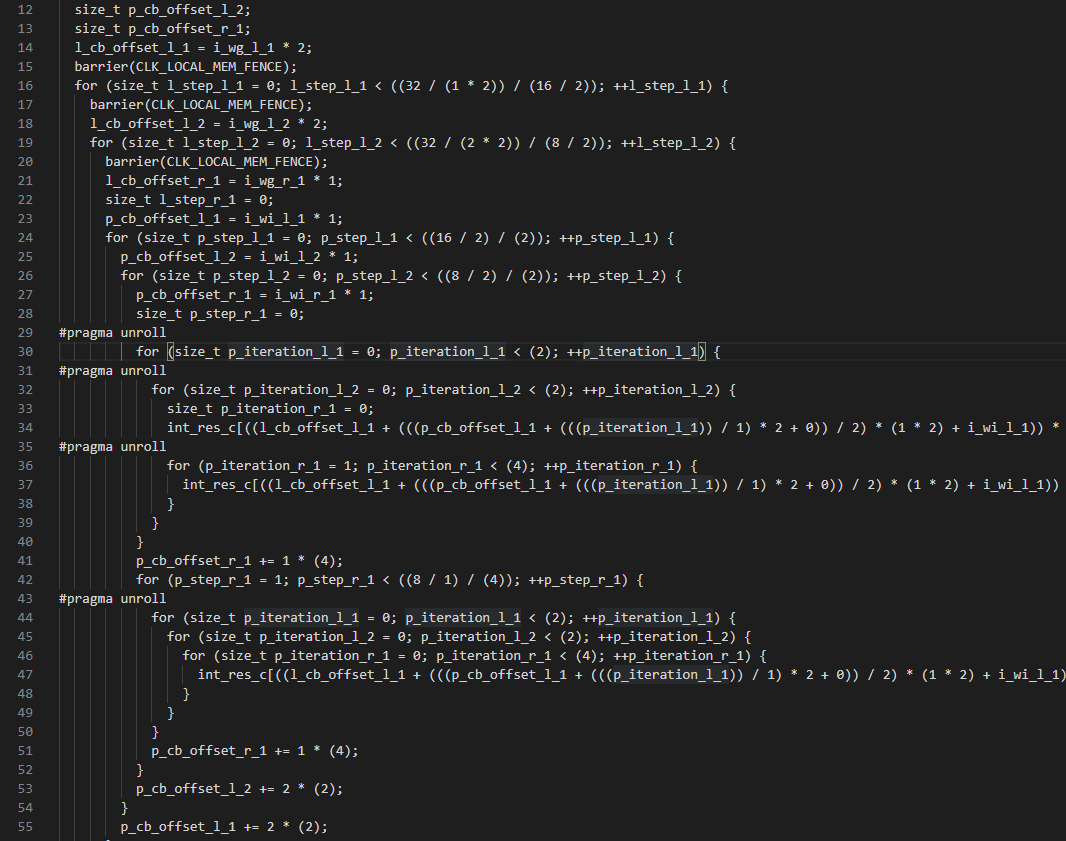
\includegraphics[width=0.9\linewidth]{images/gemm_opencl.png}
			\end{figure}
		\column{0.5\textwidth}
			\movie[height = 0.65\textwidth, width = 0.9\textwidth, poster, showcontrols] {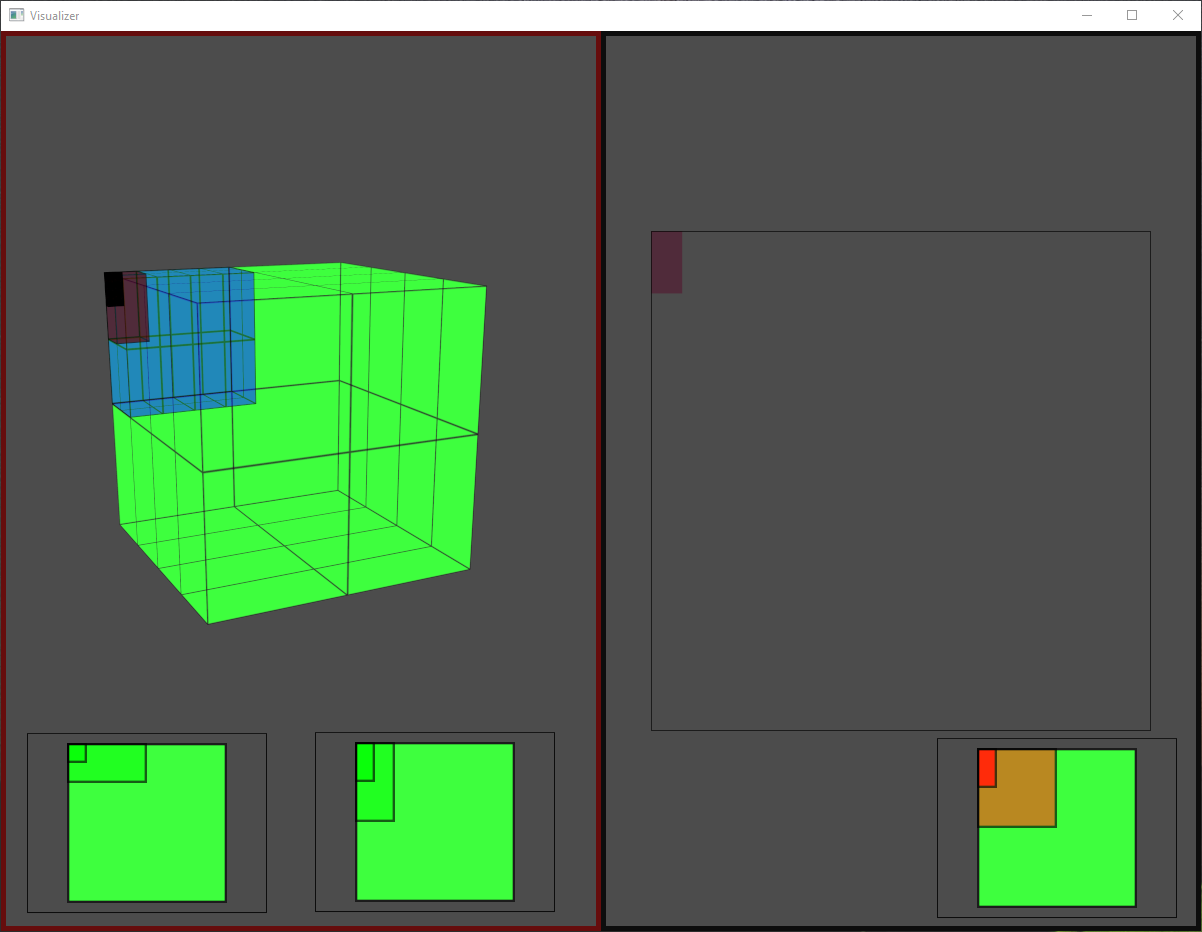
\includegraphics[height = 0.65\textwidth,width=0.9\linewidth]{images/visualizer_still.png}
			}{images/visualizer.mp4}
	\end{columns}
\end{frame}

\begin{frame}
	\frametitle{Ziel}
	Design und Implementierung eines Visualizers für komplexe daten-parallele Berechnungen:
	
	\begin{itemize}
		\item Visualizer soll funktionieren für:
		\begin{enumerate}
			\item \emph{Systemmodelle} beliebiger Tiefe: OpenCL, CUDA, OpenMP, m+-ulti-device, multi-node, etc;
			\item \emph{Berechnungen} bis zu 3 Dimensionen: DOT, GEMV, GEMM, 1D/2D/3D Stencil, etc;
			\item \emph{Konfiguration} der Berechnungen beliebiger Art: Tile Sizes, Anzahl Threads, etc.
		\end{enumerate}
		\item Visualizer soll einfach zu nutzen sein: \texttt{JSON files -> Video}
		\item Unterschied zu verwandten Arbeiten \footnote{6th Workshop on Programming and Performance Visualization Tools (ProTools) @ SC'19}: Fokus auf \emph{beliebige} jedoch \emph{einzelne} daten-parallel Berechnungen (z.B. nur GEMM) anstatt \emph{fixe} jedoch \emph{komplexe} Berechnungen (z.B. komplette Deep-Learning Graphen, in denen GEMM ein kleiner Baustein).
	\end{itemize}
\end{frame}

\begin{frame}
	\frametitle{Ansatz \& Methodik I}
	Der Visualizer soll auf folgenden Design-Entscheidungen basieren:
	
	\begin{itemize}
		\item \emph{Systemmodelle} \textbf{einheitlich} als Bäume modellieren:
		\footnote{Multi-Dimensional Homomorphisms and Their Implementation in OpenCL. Talk @ NVIDIA 2020}
		\begin{figure}
			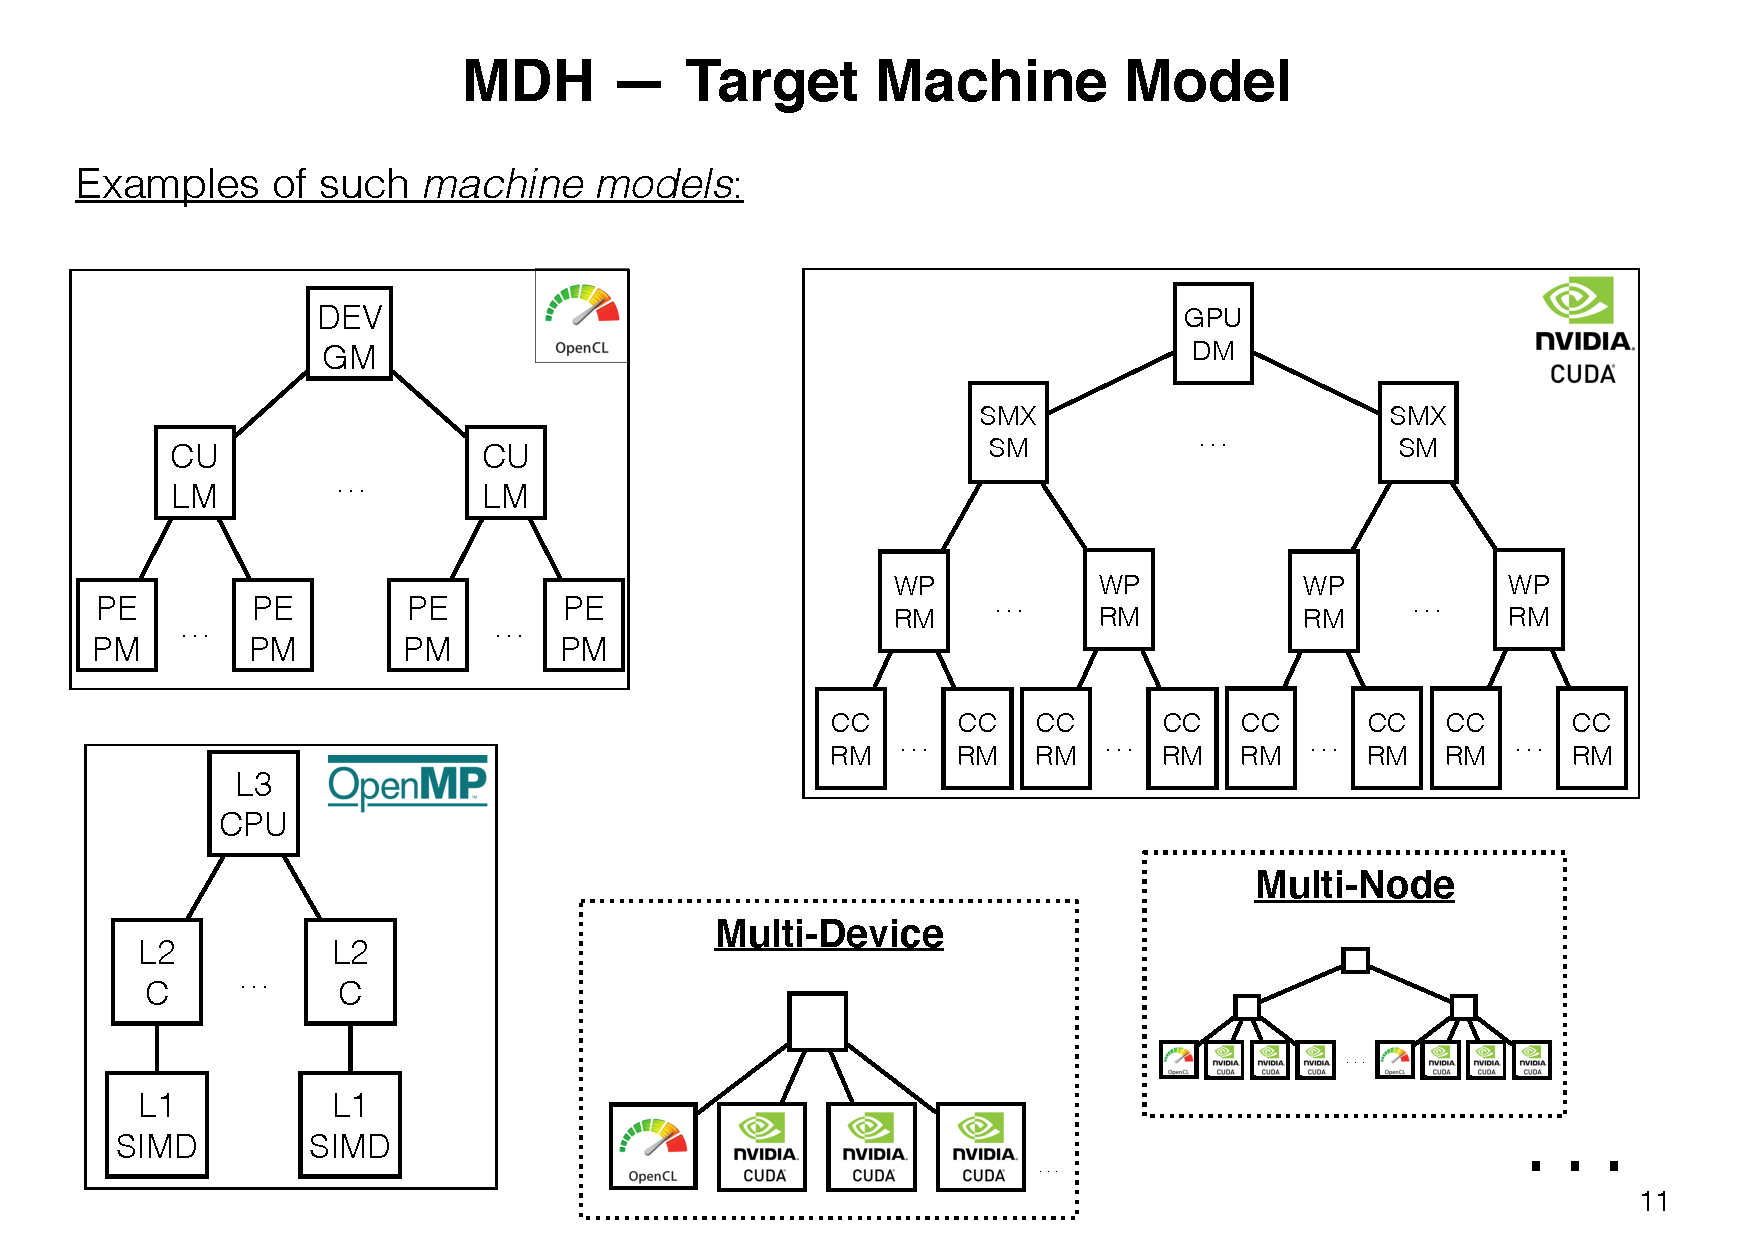
\includegraphics[width=0.6\linewidth]{images/system_models.pdf}
		\end{figure}
	\end{itemize}

\end{frame}

\begin{frame}
	\frametitle{Ansatz \& Methodik II}
	\footnotetext{Multi-Dimensional Homomorphisms and Their Implementation in OpenCL. Talk @ NVIDIA 2020} 
	\begin{itemize}
		\item \emph{Berechnungen} \textbf{einheitlich} als MDHs modellieren (da für allgemeine Daten-parallele Berechnungen):
		\footnotemark[\value{footnote}]
		\begin{figure}
			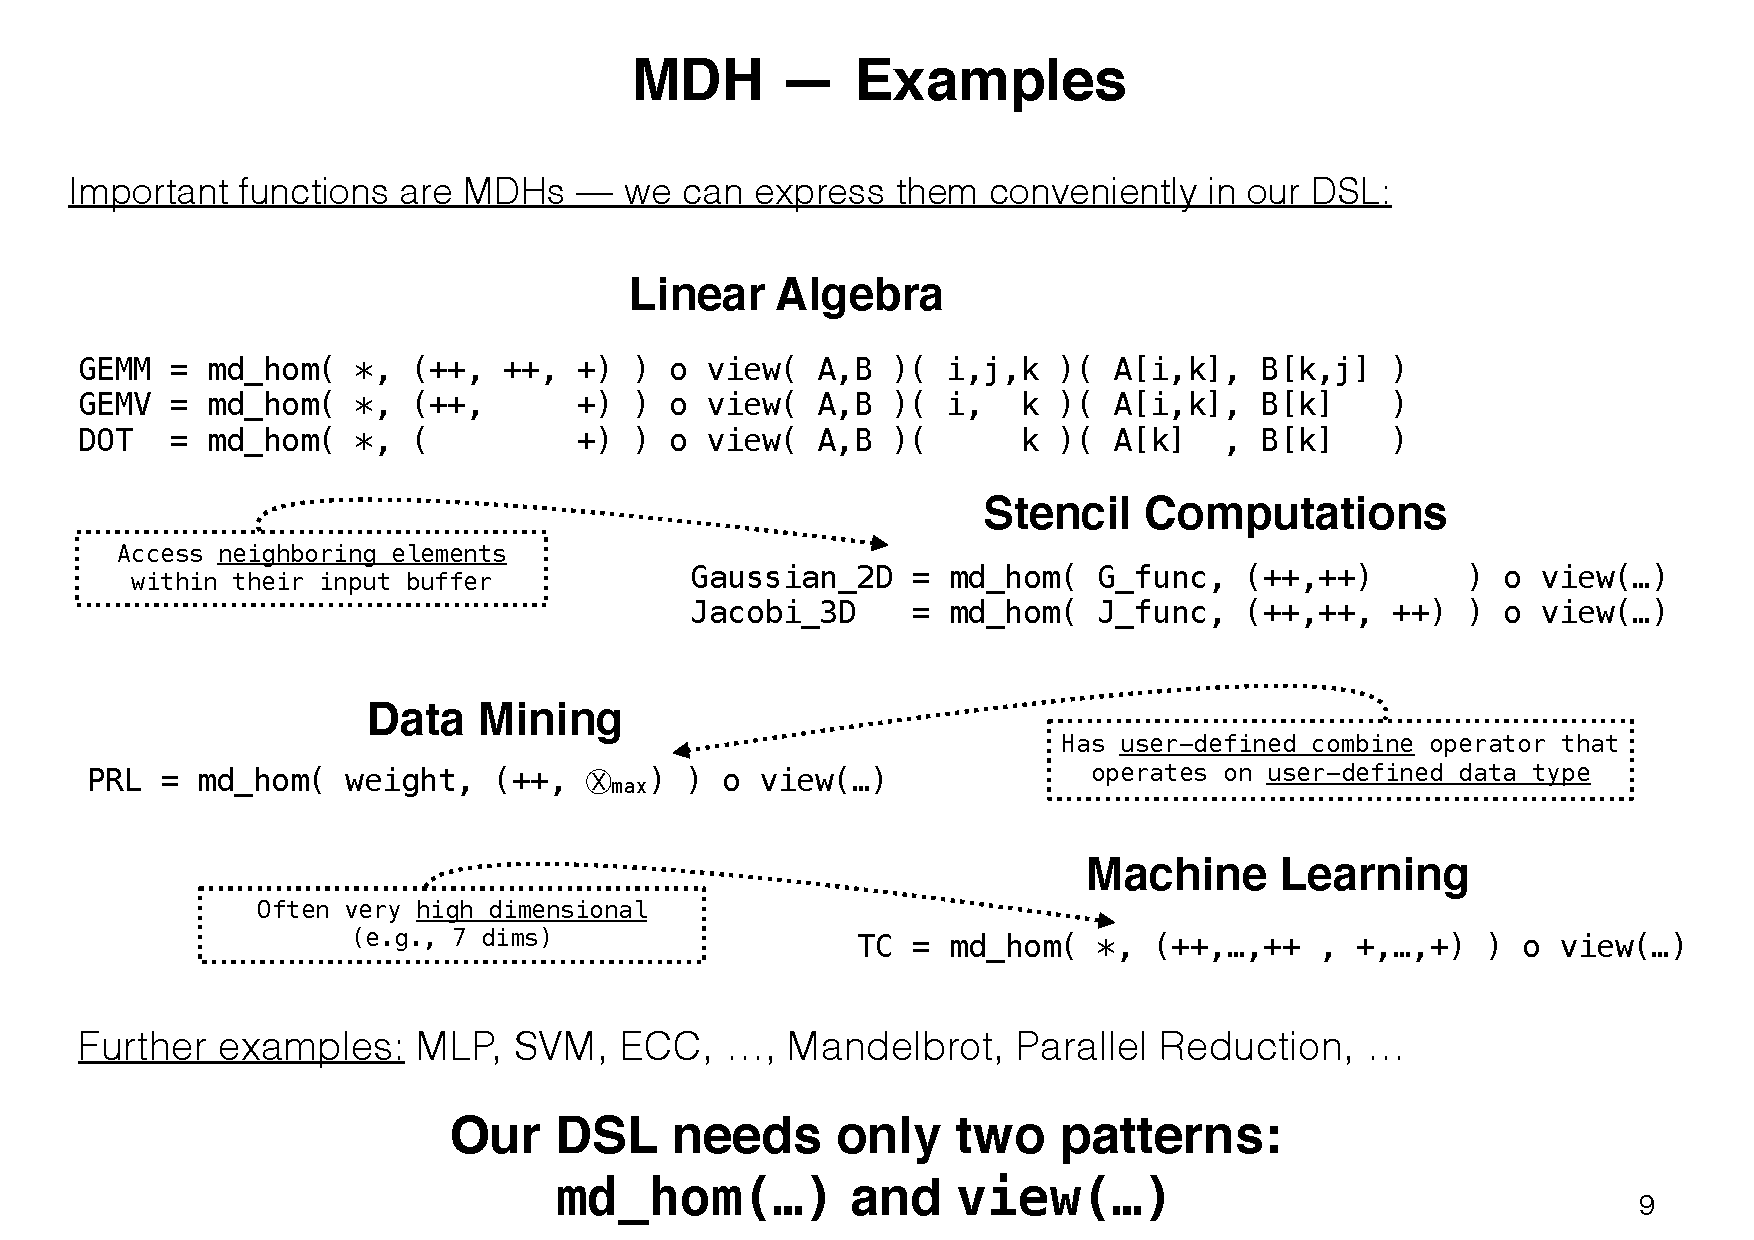
\includegraphics[width=0.6\linewidth]{images/mdhs.pdf}
		\end{figure}
	\end{itemize}
\end{frame}

\begin{frame}
	\frametitle{Ansatz \& Methodik III}
	\footnotetext{Multi-Dimensional Homomorphisms and Their Implementation in OpenCL. Talk @ NVIDIA 2020} 
	\begin{itemize}
		\item \emph{Konfiguration} \textbf{einheitlich} basierend auf MDH-Codegenierung (da Berechnungen verwandter Arbeiten dabei idR mit umfasst):
		\footnotemark[\value{footnote}]
		\begin{figure}
			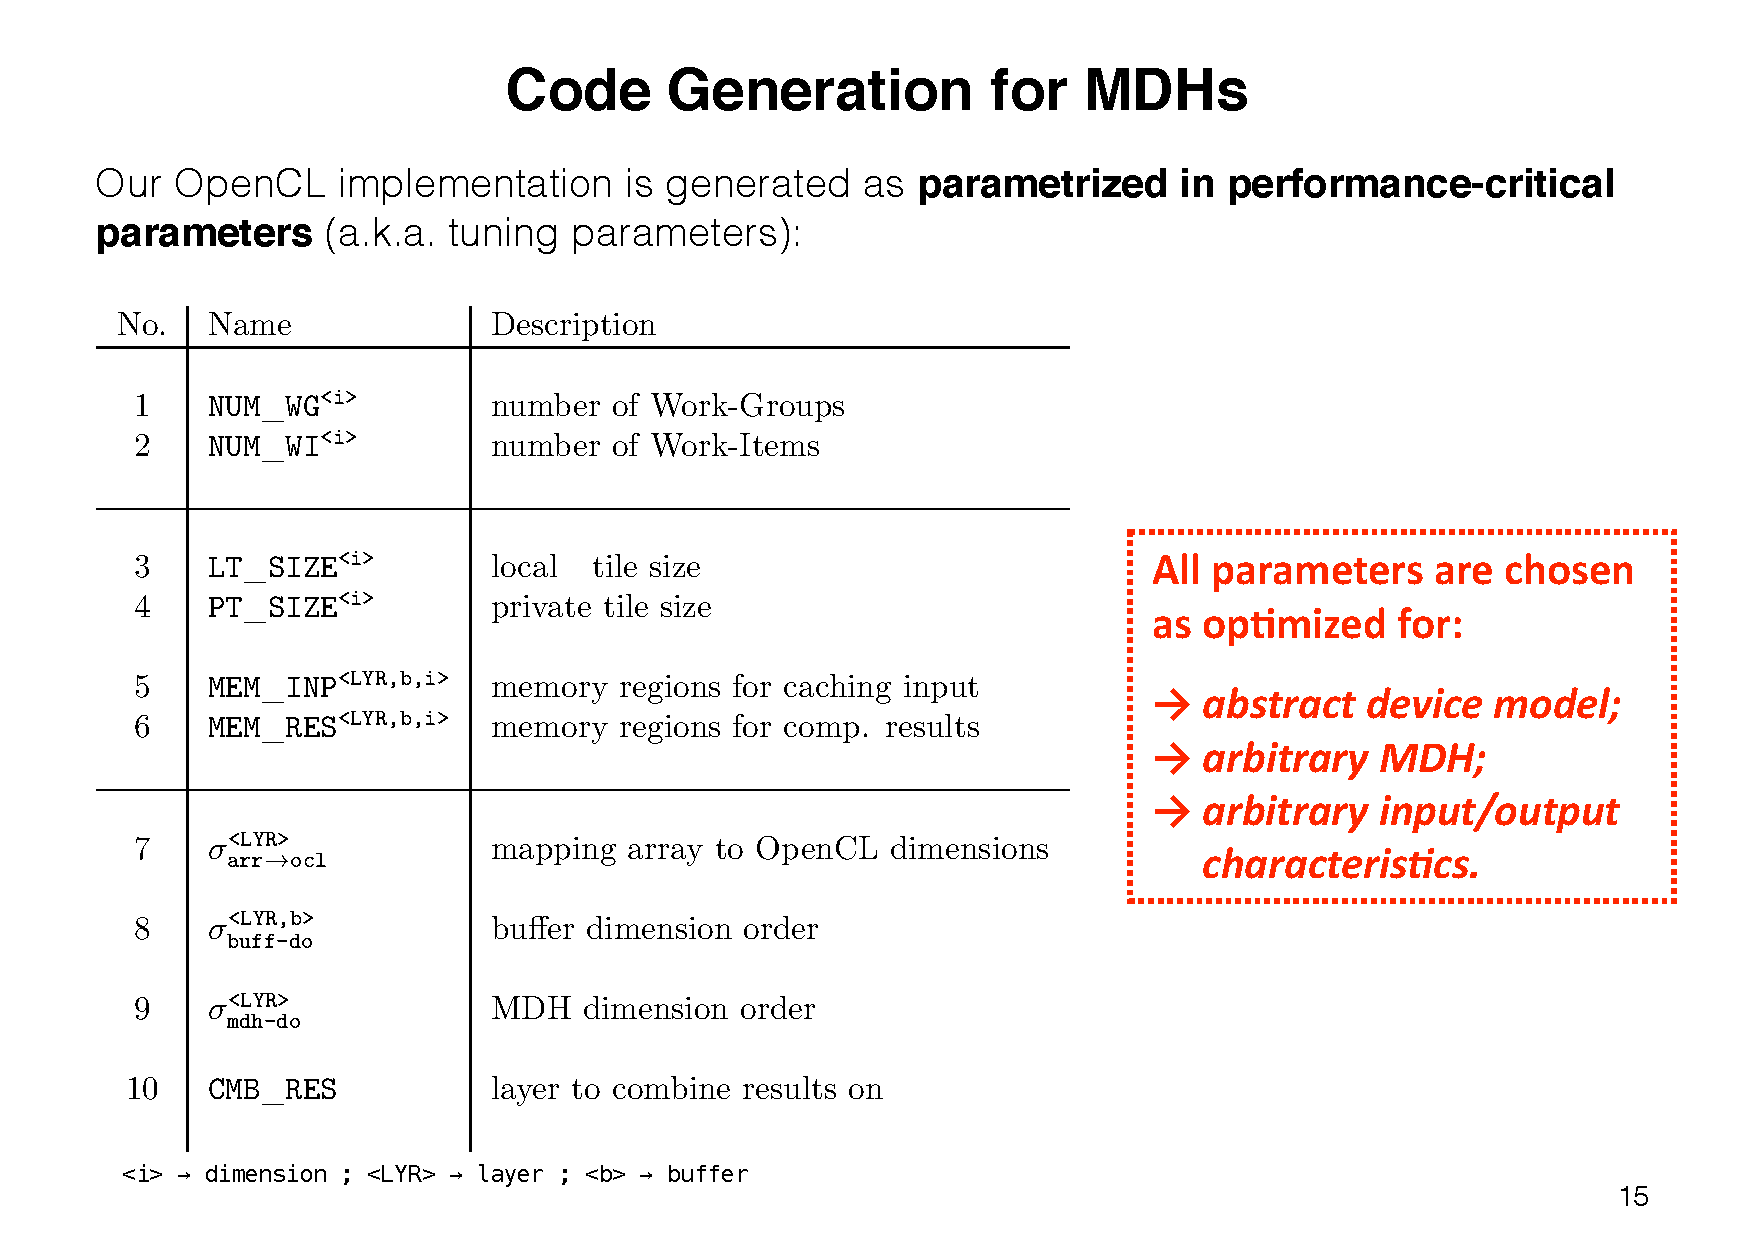
\includegraphics[width=0.6\linewidth]{images/configs.pdf}
		\end{figure}
		\framebreak
	\end{itemize}
\end{frame}

\begin{frame}
	\frametitle{Ansatz \& Methodik IV}
	Aufbau des Visualizers:
	
	\begin{figure}
		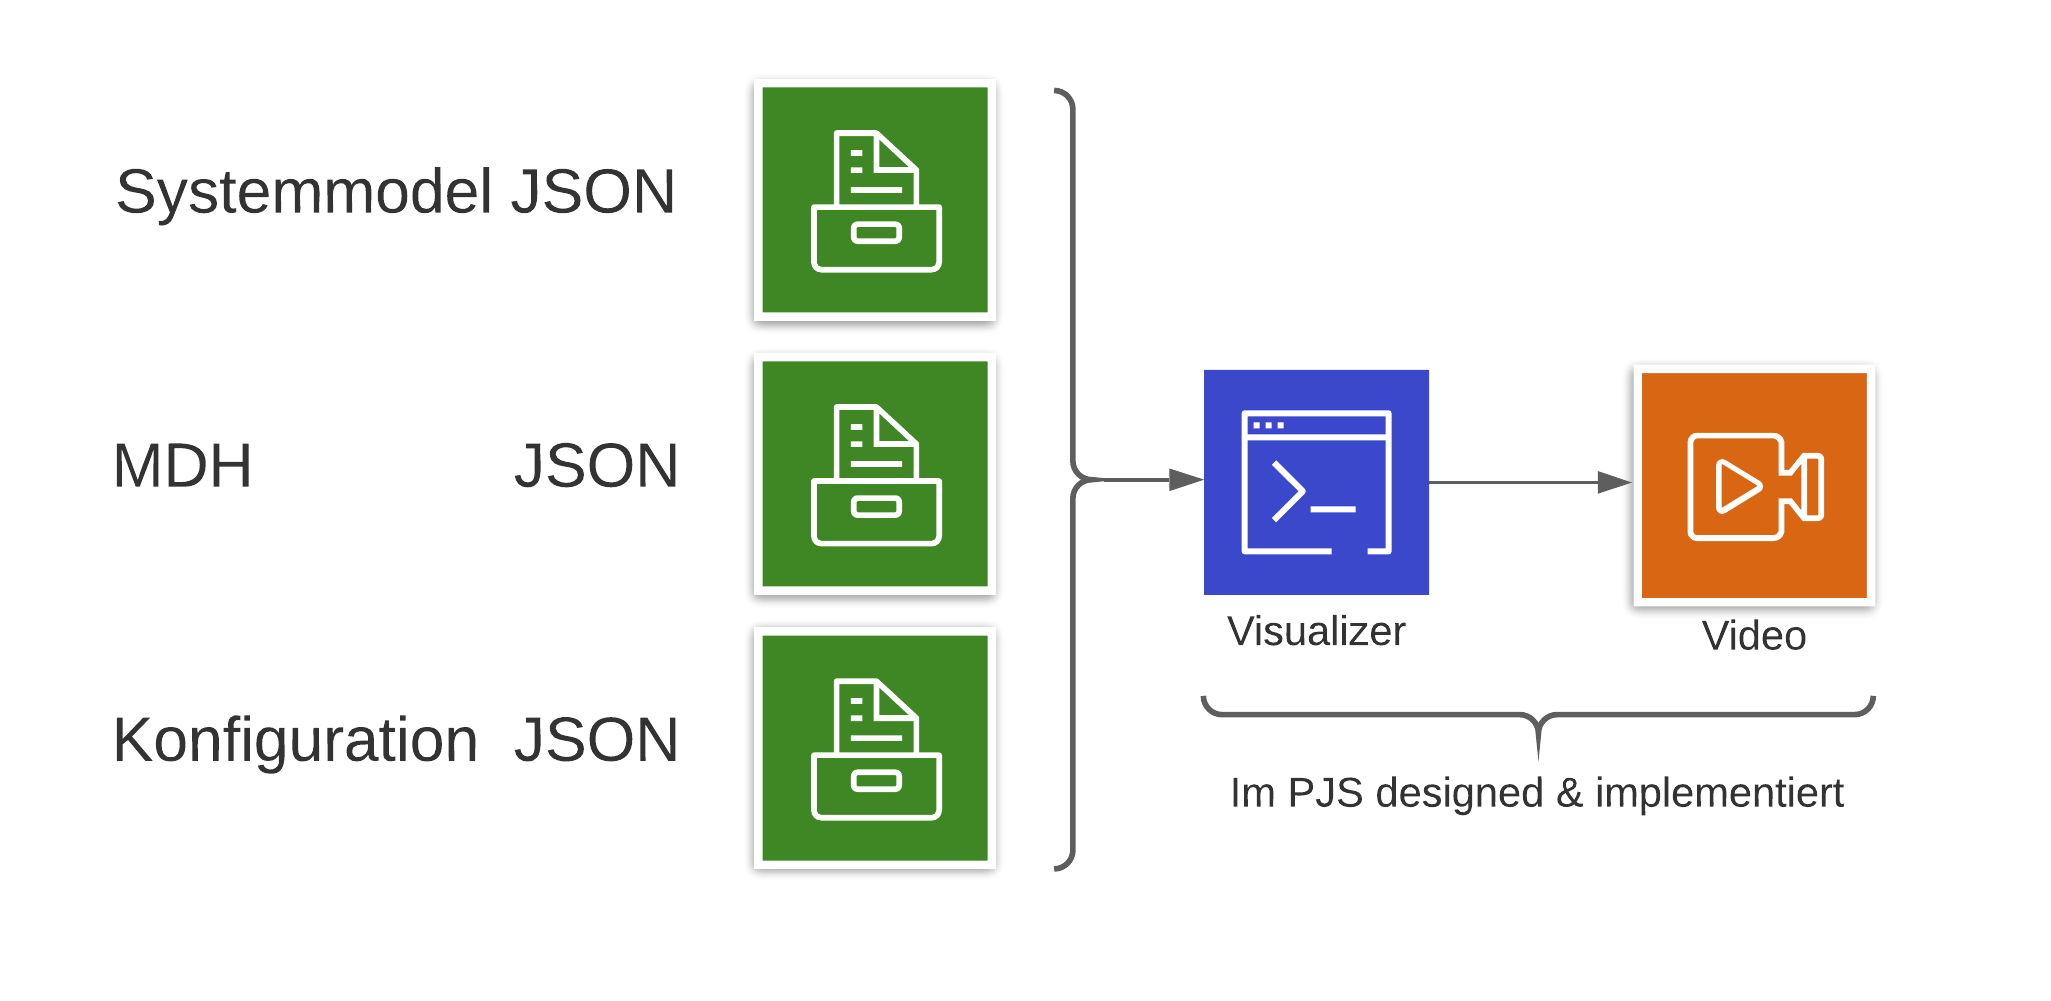
\includegraphics[scale=0.5]{images/visualizer_aufbau.png}
	\end{figure}
\end{frame}

\begin{frame}
	\frametitle{Agenda}
	Im Folgenden:
	
	\begin{enumerate}
		\item Spezifikation der JSONs:
		\begin{enumerate}
			\item Systemmodel
			\item MDH
			\item Konfiguration
		\end{enumerate}
		\item Design \& Implementierung des Visualizers
	\end{enumerate}
\end{frame}

\begin{frame}[allowframebreaks]
	\frametitle{1.1 Spezifikation: Systemmodelle}
	Systemmodelle als JSON files:\\
	Die Baumhierarchie des Systemmodells wird als JSON files dargestellt.
	
	\bigskip
	
	Beispiele:
	\begin{itemize}
		\item OpenCL Baum:
		\lstinputlisting[style=context, basicstyle=\fontsize{1}{2}\selectfont\ttfamily]{listings/model_opencl.txt}
		\framebreak
		\item CUDA Baum:
		\lstinputlisting[style=context, basicstyle=\fontsize{4}{6}\selectfont\ttfamily]{listings/model_cuda.txt}
		\framebreak
		\item Multi-Dev Baum:
		\lstinputlisting[style=context, basicstyle=\fontsize{4}{6}\selectfont\ttfamily]{listings/model_multi_dev.txt}
	\end{itemize}
\end{frame}

\begin{frame}[allowframebreaks]
	\frametitle{1.2 Spezifikation: MDH}
	MDHs als JSON files:\\
	Der MDH-Ausdruck (\emph{md\_hom()} und \emph{view()}) wird als einer JSON Datei dargestellt.
	
	\bigskip
	
	Beispiele:
	\begin{itemize}
		\item GEMM:
		\lstinputlisting[style=context, basicstyle=\fontsize{5}{7}\selectfont\ttfamily]{listings/mdh_gemm.txt}
		\framebreak
		\item Stencil:
		\lstinputlisting[style=context, basicstyle=\fontsize{5}{7}\selectfont\ttfamily]{listings/mdh_stencil.txt}
	\end{itemize}
\end{frame}

\begin{frame}
	\frametitle{1.3 Spezifikation: Konfiguration}
	Konfiguration als JSON files:\\
	Die Konfiguration (Tuning-Parameter) werden pro Schicht als einer JSON Datei dargestellt.
	
	\bigskip
	
	Beispiel:\\
	
	\begin{table}
		\begin{tabular}{l | c | c | c | c }
			Layer & ... & Tile Size & Anzahl Threads & ... \\
			\hline \hline
			Layer 0 & ... & (32, 32, 32) & (1, 1, 1) & ... \\
			\hline
			... & ... & ... & ... & ... \\
		\end{tabular}
		\caption{Beispiel Konfiguration}
	\end{table}
	
	\lstinputlisting[style=context, basicstyle=\fontsize{5}{7}\selectfont\ttfamily]{listings/tps.txt}
\end{frame}

\begin{frame}
	\frametitle{2. Design \& Implementierung: Visualizer}
	Aufbau des Visualizers:
	\begin{figure}
		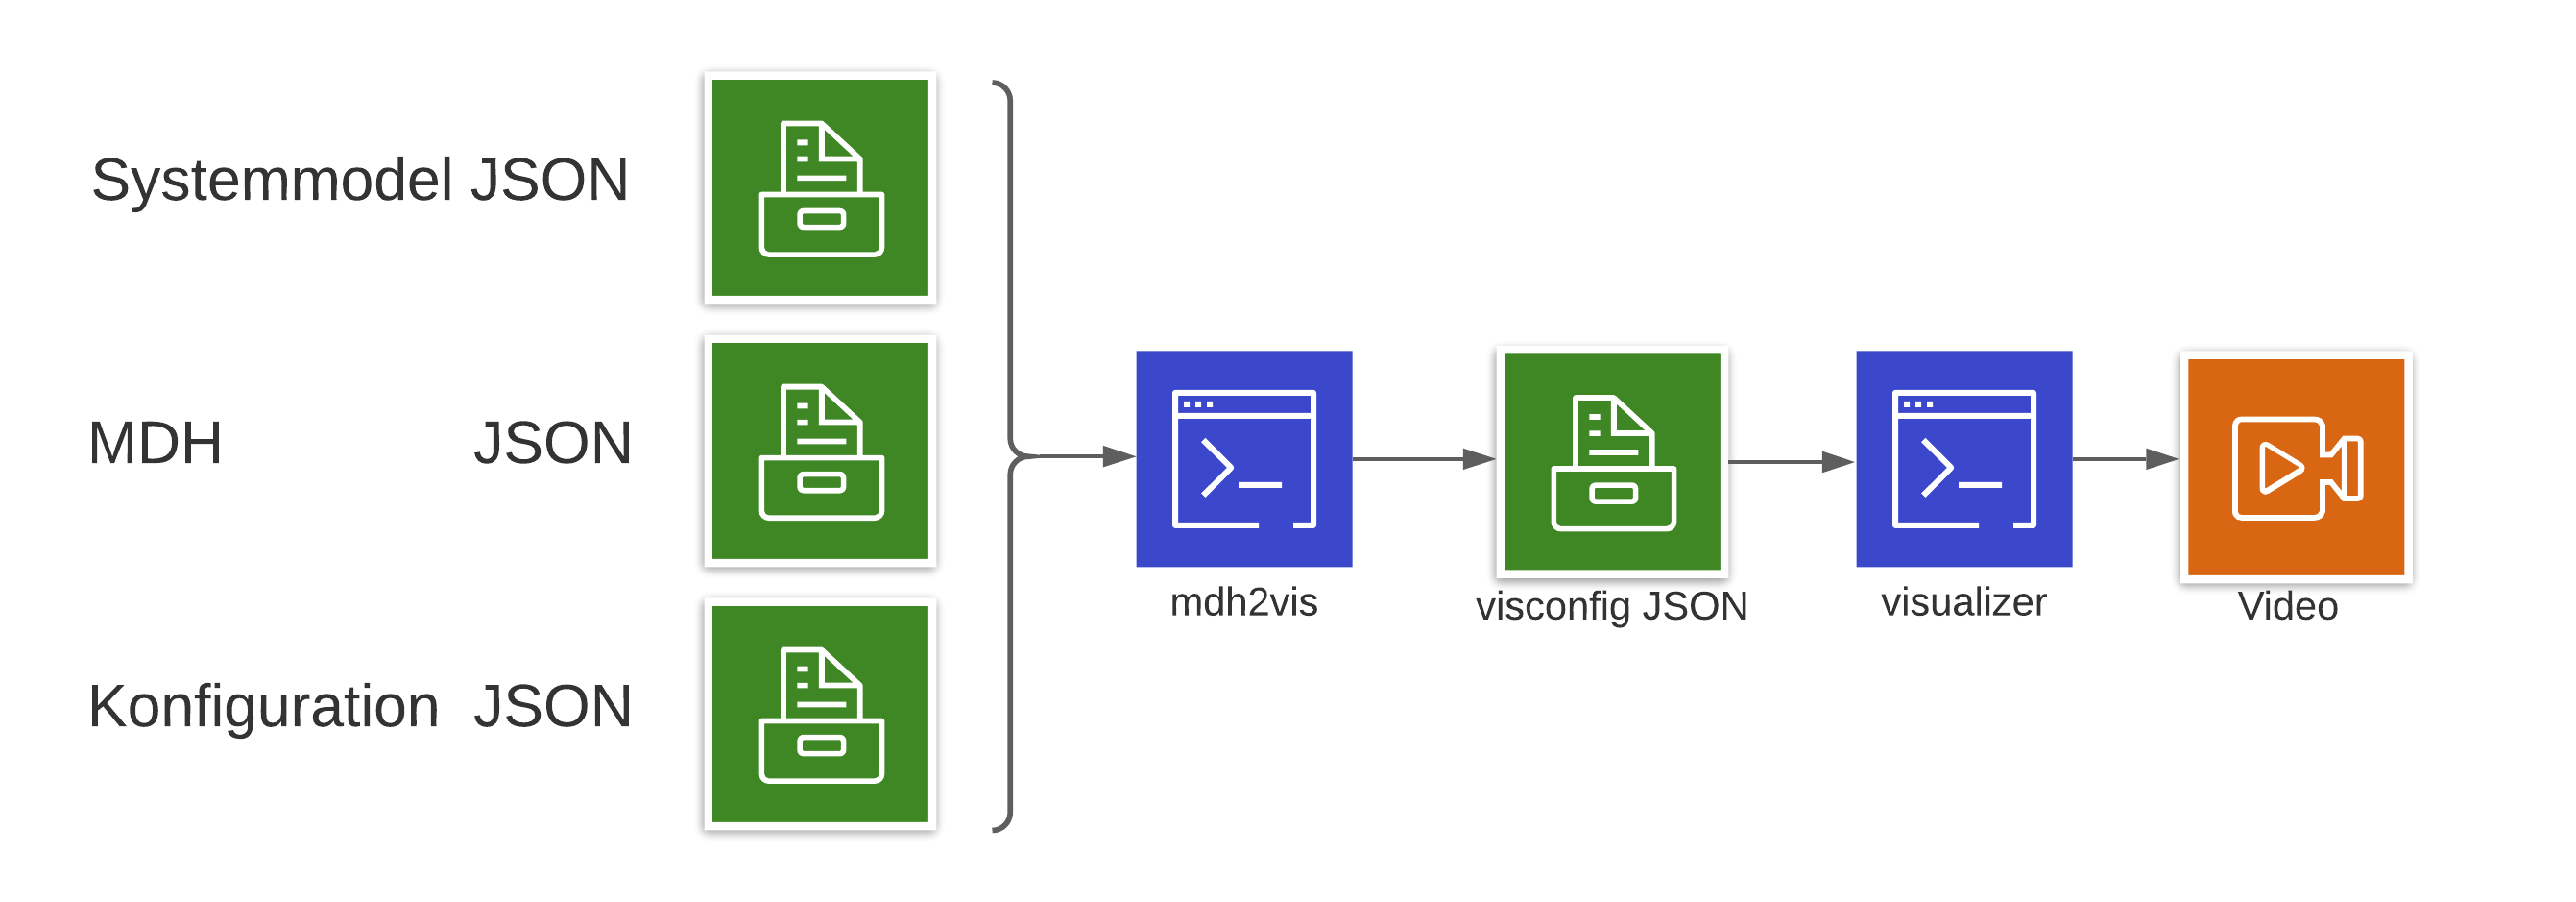
\includegraphics[scale=0.5]{images/visualizer_aufbau_praezise.png}
	\end{figure}
	
	visconfig JSON: Textuelle Repräsentation der MDH-Konfiguration seitens des Visualizers..\\
	mdh2vis: Übersetzer von \texttt{Systemmodel+MDH+Konfiguration JSONs} zu \texttt{visconfig JSON} (straightforward)
\end{frame}

\begin{frame}
	\frametitle{2. Spezifikation: visconfig JSON}
	Repräsentation einer verarbeiteten MDH-Konfiguration, welches von den visualizer eingelesen werden kann:
	\begin{itemize}
		\item Festes Schema für beliebige MDH-Konfigurationen.
		\item Die Konzepte einer MDH-Konfiguration (wie die Tuning-Parameter und Speicherschichten) gehen verloren.
		\item Stattdessen werden neue Konzepte aus dem visualizer eingeführt.
		\item Ist rein deklarativ und somit einfach erweiterbar.
	\end{itemize}
\end{frame}

\begin{frame}
	\frametitle{2. Spezifikation: mdh2vis I}
	\begin{columns}
		\column{0.5\textwidth}
		MDH-Konfiguration JSONs:
		\begin{figure}
			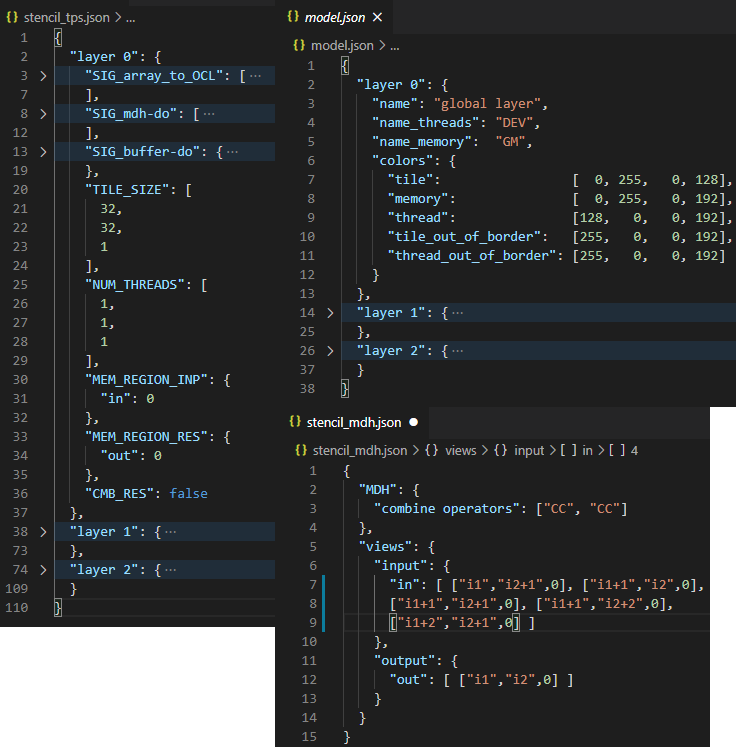
\includegraphics[width=0.9\linewidth]{images/konfiguration_stencil.png}
		\end{figure}
		\column{0.5\textwidth}
		visconfig JSON:
		\begin{figure}
			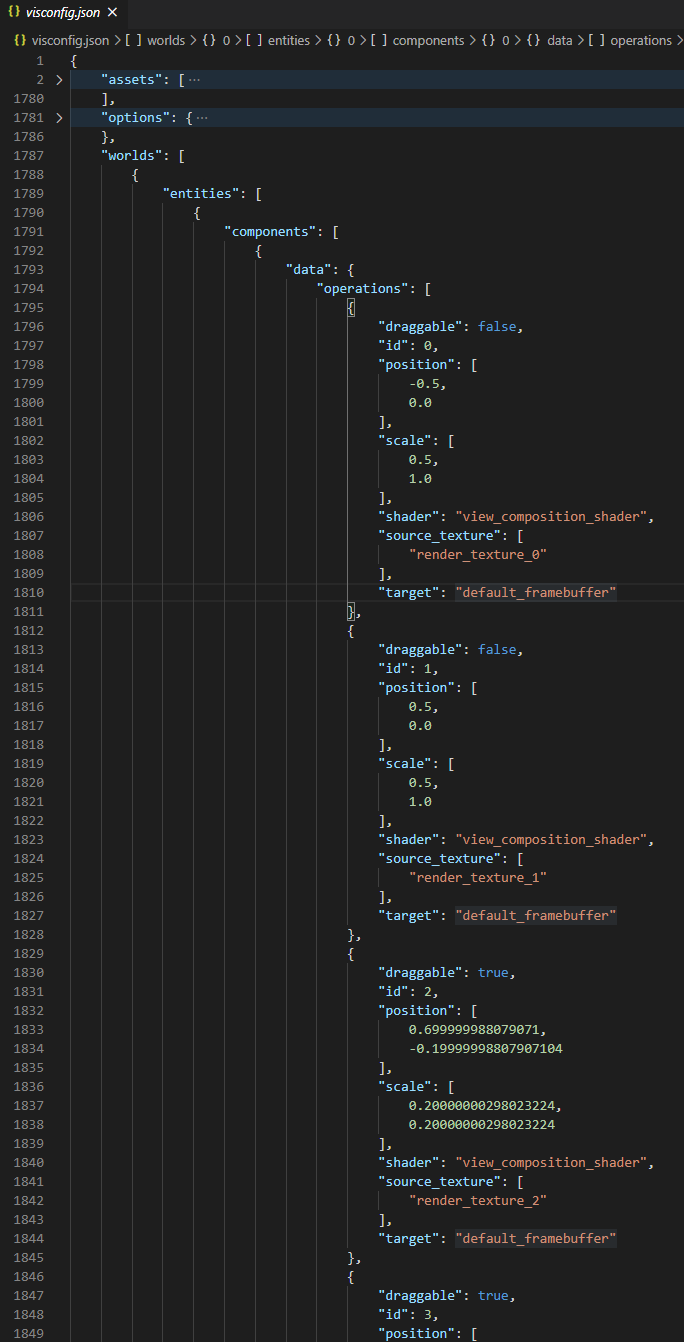
\includegraphics[scale=0.18]{images/konfiguration_stencil_visualizer.png}
		\end{figure}
	\end{columns}
\end{frame}

\begin{frame}
	\frametitle{2. Spezifikation: mdh2vis II}
	\begin{columns}
		\column{0.5\textwidth}
		Systemmodell JSON:
		\begin{figure}
			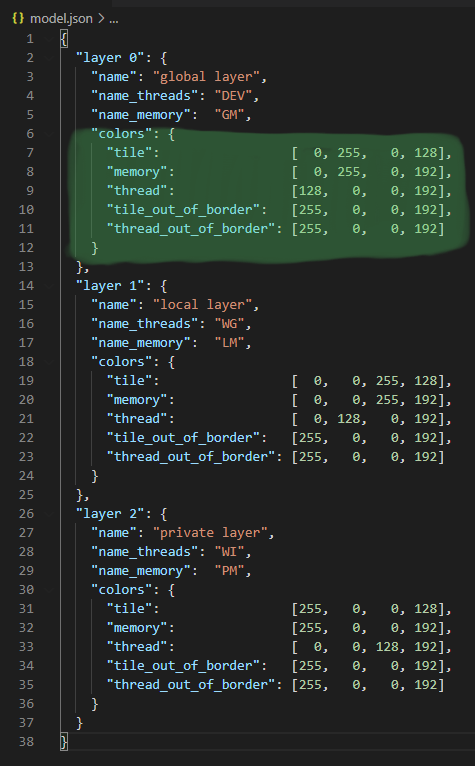
\includegraphics[width=0.6\linewidth]{images/gemm_model.png}
		\end{figure}
		\column{0.5\textwidth}
		visconfig JSON:
		\begin{figure}
			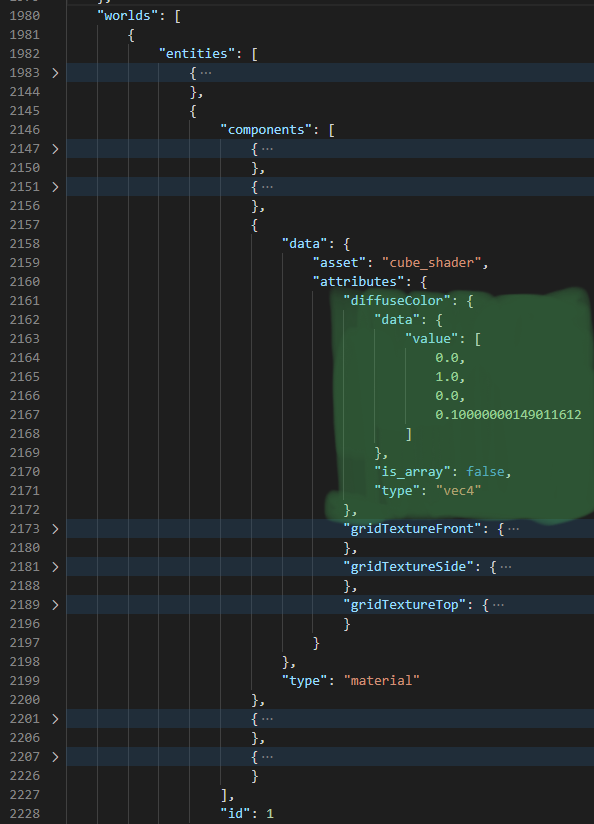
\includegraphics[width=0.7\linewidth]{images/gemm_model_vis.png}
		\end{figure}
	\end{columns}
\end{frame}

\begin{frame}
	\frametitle{2. Spezifikation: mdh2vis III}
	\begin{columns}
		\column{0.5\textwidth}
		Berechnung JSON:
		\begin{figure}
			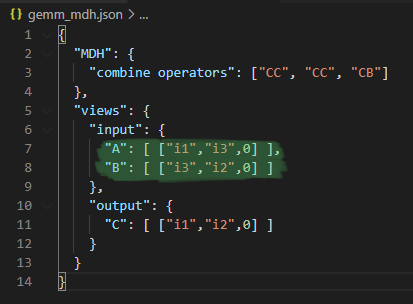
\includegraphics[width=\linewidth]{images/gemm_mdh.png}
		\end{figure}
		\column{0.5\textwidth}
		visconfig JSON:
		\begin{figure}
			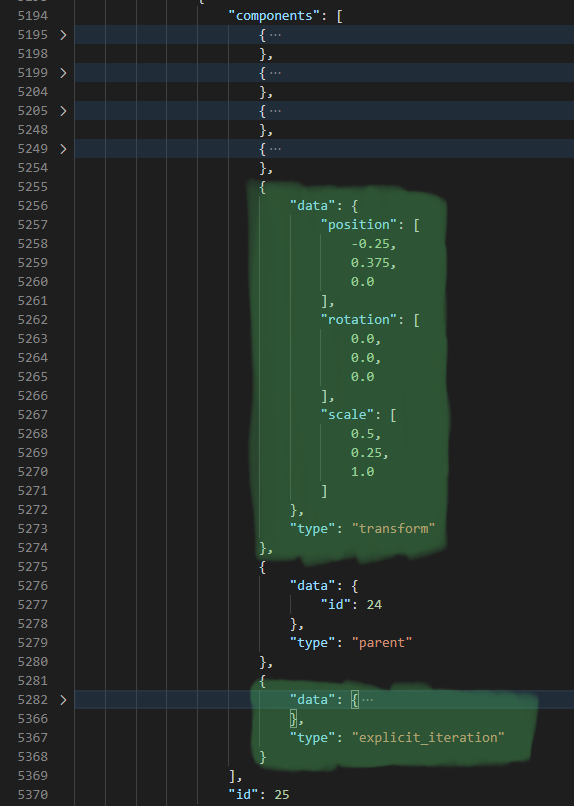
\includegraphics[width=0.7\linewidth]{images/gemm_mdh_vis.png}
		\end{figure}
	\end{columns}
\end{frame}

\begin{frame}
	\frametitle{2. Spezifikation: mdh2vis IV}
	\begin{columns}
		\column{0.5\textwidth}
		Konfiguration JSON:
		\begin{figure}
			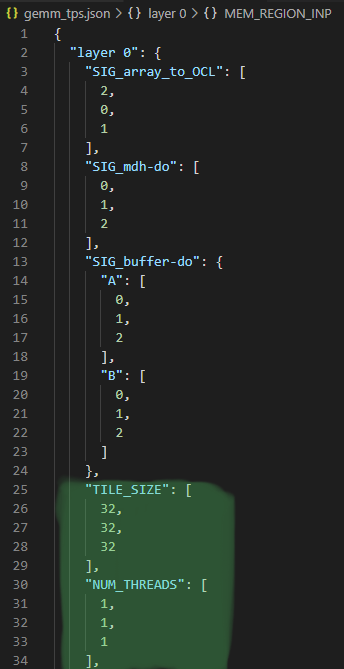
\includegraphics[width=0.54\linewidth]{images/gemm_tps.png}
		\end{figure}
		\column{0.5\textwidth}
		visconfig JSON:
		\begin{figure}
			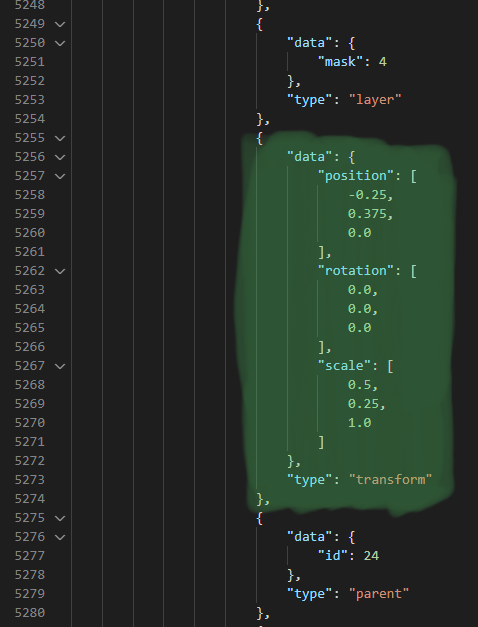
\includegraphics[width=0.8\linewidth]{images/gemm_tps_vis.png}
		\end{figure}
	\end{columns}
\end{frame}

\begin{frame}[allowframebreaks]
	\frametitle{2. Spezifikation: visualizer}
	\begin{columns}
		\column{0.5\textwidth}
		Der visualizer läuft in einer Endlosschleife:
		\bigskip
		\begin{itemize}
			\item Initialisierung durchs einlesen der visconfig JSON.
			\item Zustand aktualisieren.
			\item Zustand anzeigen.
		\end{itemize}
		\column{0.5\textwidth}
		\begin{figure}
			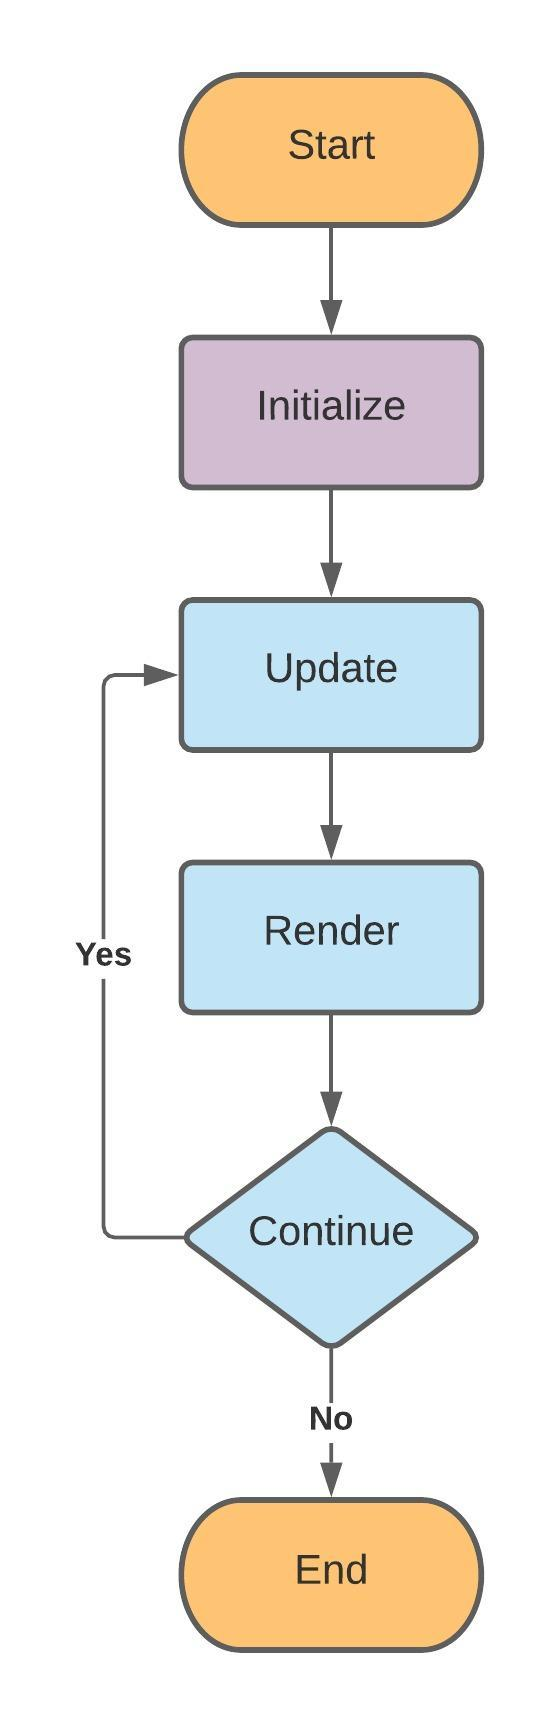
\includegraphics[scale=0.45]{visualizer_render_loop.jpg}
		\end{figure}
	\end{columns}

	\framebreak
	
	Update:
	\bigskip
	\begin{itemize}
		\item Das Programm speichert den Zustand aller sichtbaren Objekte.
		\item Ein Objekt kann mehrere Attribute besitzen: Position, Form, Farbe, etc.
		\item Dieser Zustand wird durch eine Menge von Prozeduren transformiert.
		\item Diese Prozeduren funktionieren unabhängig von der MDH-Konfiguration.
	\end{itemize}
	
	\framebreak
	
	\begin{figure}
		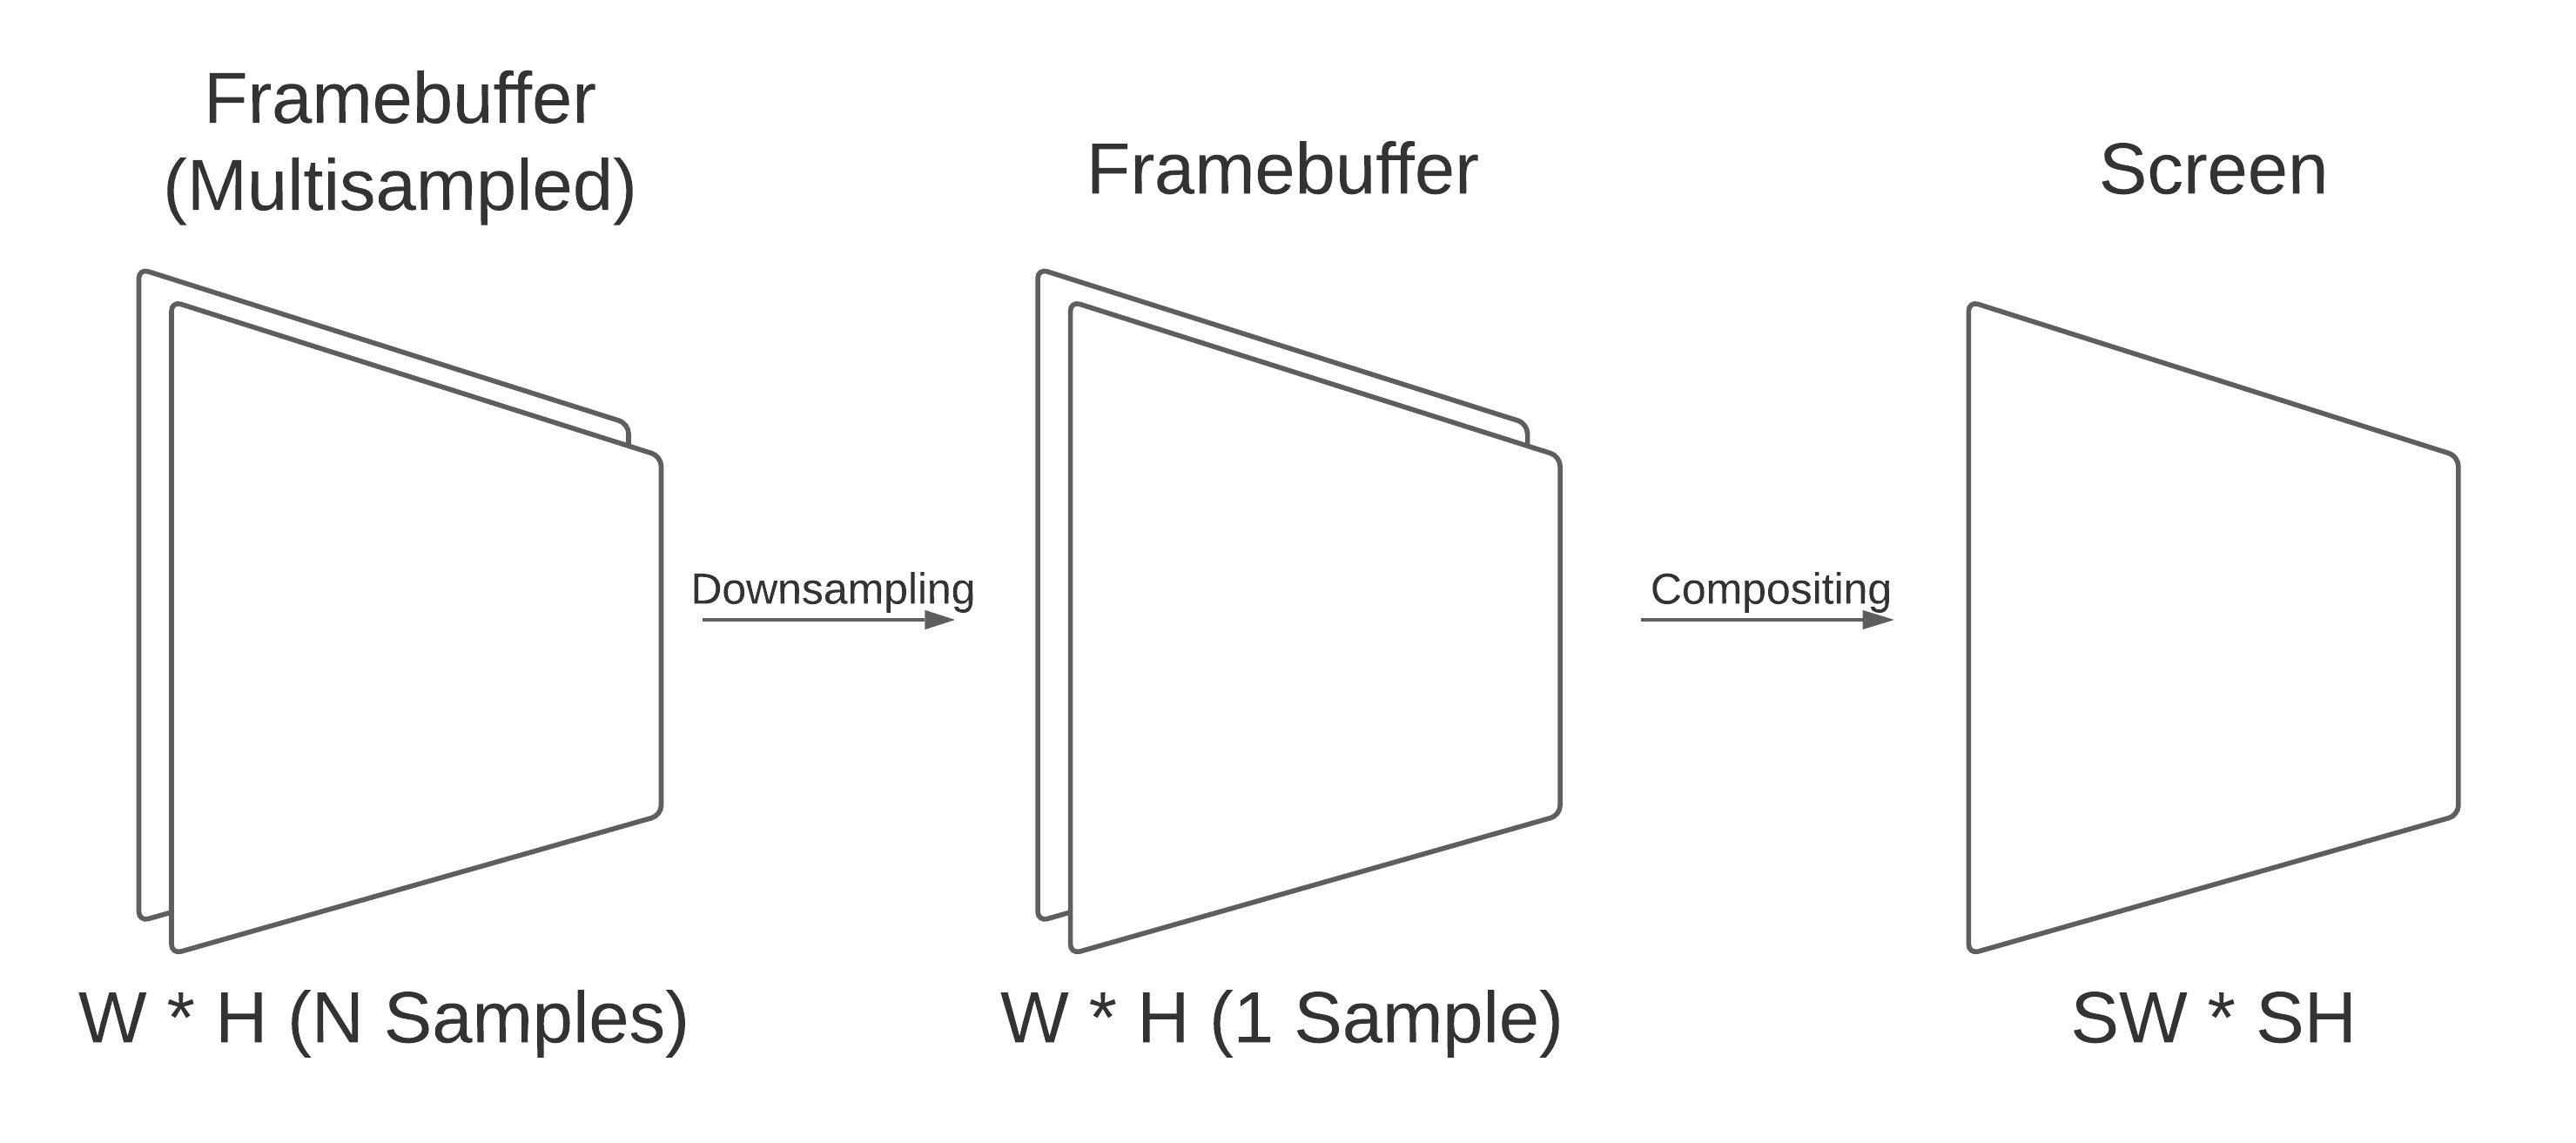
\includegraphics[scale=0.3]{render_pipeline.jpg}
	\end{figure}
	
	Zeichnen:
	\bigskip
	\begin{itemize}
		\item Zum zeichnen wird die OpenGL Bibliothek verwendet.
		\item Alle Views (MDH-View, Ausgabe-View, Input-/Output-View) werden in unterschiedliche Framebuffer (oder Bildausgabepuffer) gezeichnet. Diese werden kombiniert und auf den Bildschirm angezeigt.
		\item Die einzelnen Views können mit der Maus bewegt werden.
	\end{itemize}
\end{frame}

\begin{frame}[allowframebreaks, fragile]
	\frametitle{Aktueller Stand \& Ausblick}
	Die Visualisierung ist noch \textcolor{blue}{nicht vollständig}:\\
	MDH:
	\lstinputlisting[style=context]{listings/gemm_mdh.json}
	\framebreak
	Konfiguration:
	\lstinputlisting[style=context]{listings/gemm_tps.json}
	\framebreak
	Systemmodel:
	\lstinputlisting[style=context]{listings/model.json}
	\framebreak
	
	Einschränkungen:
	\begin{itemize}
		\item Teil Size muss glatt durcheinander Teilbar sein.
		\item Performance ist von der Größe der Eingabedaten abhängig.
	\end{itemize}
\end{frame}

\begin{frame}
	\centering \Huge
	\emph{Danke fürs Zuhören.}
\end{frame}

\end{document}

% vi: tw=100